
\documentclass[a4paper,12pt,titlepage,final]{article}
% Language setting
% Replace `english' with e.g. `spanish' to change the document language
\usepackage[english, russian]{babel}

% Set page size and margins
% Replace `letterpaper' with `a4paper' for UK/EU standard size
\usepackage[letterpaper,top=2cm,bottom=2cm,left=3cm,right=3cm,marginparwidth=1.75cm]{geometry}
\usepackage{float}
% Useful packages
\usepackage{amsmath}
\usepackage{graphicx}
\usepackage[colorlinks=true, allcolors=blue]{hyperref}


\usepackage[T1,T2A]{fontenc}     % форматы шрифтов
\usepackage[utf8x]{inputenc}     % кодировка символов, используемая в данном файле
\usepackage{amsmath}      % для настройки размера полей
\usepackage{indentfirst}         % для отступа в первом абзаце секции
\begin{document}
\begin{titlepage}
    \begin{center}
    {\small \sc Московский Государственный Университет имени М. В. Ломоносова \\
    Факультет Вычислительной Математики и Кибернетики\\}
    \vfill
    
    {\large \bf Отчет по практическому заданию по курсу Распределённые системы\\}
    \end{center}
    \begin{flushright}
    \vfill {
    Воробьев Евгений\\
    428 группа\\
    }
    \end{flushright}
    \begin{center}
    \vfill
    {\small Москва\\2023}
    \end{center}
    \par
\end{titlepage}

% Автоматически генерируем оглавление на отдельной странице
\tableofcontents

\newpage
\section{Задача 1}
\begin{itemize}
\item Разработать программу которая реализует заданный алгоритм. 
\item Получить временную оценку работы алгоритма.
\end{itemize}

\subsection{Описание}\par
Все 25 процессов, находящихся на разных ЭВМ сети, одновременно выдали запрос на вход в критическую секцию. Реализовать программу, использующую древовидный маркерный алгоритм для прохождения всеми процессами критических секций.
Критическая секция:
\begin{verbatim}
<проверка наличия файла “critical.txt”>;
if (<файл “critical.txt” существует>) {
<сообщение об ошибке>;
<завершение работы программы>;
} else {
<создание файла “critical.txt”>;
sleep (<случайное время>);
<уничтожение файла “critical.txt”>;
}    
\end{verbatim}
Для передачи маркера использовать средства MPI.
Получить временную оценку работы алгоритма. Оценить сколько времени потребуется, если маркером владеет нулевой процесс. Время старта (время «разгона» после получения доступа к шине для передачи сообщения) равно 100, время передачи байта равно 1 (Ts=100,Tb=1). Процессорные операции, включая чтение из памяти и запись в память, считаются бесконечно быстрыми.
\subsection{Реализация}
\begin{figure}[h!]
  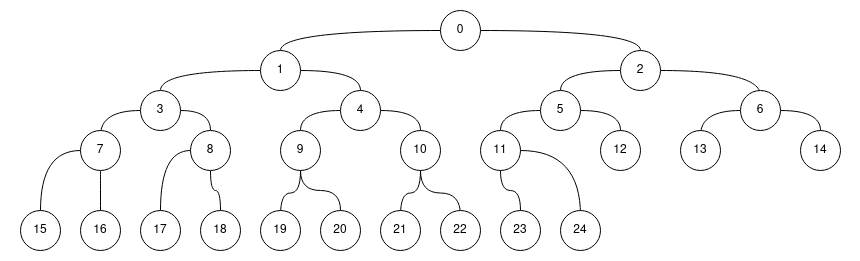
\includegraphics[width=1\linewidth]{marker.png}
  \caption{Схема системы передачи маркера}
  \label{fig:marker}
\end{figure}
Маркер передается в последовательности: 0 -> 1 -> 3 -> 7 -> 15 -> 7 -> 16 -> 7 -> 3 -> 8 ...\par
Итого сообщений передачи маркера с запросом – 21, маркера без запроса – 24, всего передач маркера – 45.\par
(Lz - запрос, Lm - маркер; считаем эти сообщения равными 4 байтам)\par
Таким образом, (Ts+Tb*Lz)*21+(Ts+Tb*Lm)*45 = 6864.
\subsection{Результаты}
\begin{verbatim}
21 requested marker from 10.
12 requested marker from 5.
7 requested marker from 3.
24 requested marker from 11.
2 requested marker from 0.
8 requested marker from 3.
15 requested marker from 7.
13 requested marker from 6.
17 requested marker from 8.
14 requested marker from 6.
20 requested marker from 9.
11 requested marker from 5.
0 aqcuared the marker.
Process 0 started working. It'll finish in 7 second(s).
4 requested marker from 1.
10 requested marker from 4.
1 requested marker from 0.
5 requested marker from 2.
9 requested marker from 4.
3 requested marker from 1.
22 requested marker from 10.
16 requested marker from 7.
6 requested marker from 2.
19 requested marker from 9.
18 requested marker from 8.
23 requested marker from 11.
Process 0 finished working.
0 sending marker to 1.
0 requested marker from 1.
1 aqcuared the marker.
Process 1 started working. It'll finish in 2 second(s).
Process 1 finished working.
1 sending marker to 3.
1 requested marker from 3.
3 aqcuared the marker.
Process 3 started working. It'll finish in 9 second(s).
Process 3 finished working.
3 sending marker to 7.
3 requested marker from 7.
7 aqcuared the marker.
Process 7 started working. It'll finish in 6 second(s).
Process 7 finished working.
7 sending marker to 15.
7 requested marker from 15.
15 aqcuared the marker.
Process 15 started working. It'll finish in 6 second(s).
Process 15 finished working.
15 sending marker to 7.
7 aqcuared the marker.
7 sending marker to 16.
7 requested marker from 16.
16 aqcuared the marker.
Process 16 started working. It'll finish in 7 second(s).
Process 16 finished working.
16 sending marker to 7.
7 aqcuared the marker.
7 sending marker to 3.
3 aqcuared the marker.
3 sending marker to 8.
3 requested marker from 8.
8 aqcuared the marker.
Process 8 started working. It'll finish in 4 second(s).
Process 8 finished working.
8 sending marker to 17.
8 requested marker from 17.
17 aqcuared the marker.
Process 17 started working. It'll finish in 2 second(s).
Process 17 finished working.
17 sending marker to 8.
8 aqcuared the marker.
8 sending marker to 18.
8 requested marker from 18.
18 aqcuared the marker.
Process 18 started working. It'll finish in 9 second(s).
Process 18 finished working.
18 sending marker to 8.
8 aqcuared the marker.
8 sending marker to 3.
3 aqcuared the marker.
3 sending marker to 1.
1 aqcuared the marker.
1 sending marker to 4.
1 requested marker from 4.
4 aqcuared the marker.
Process 4 started working. It'll finish in 10 second(s).
Process 4 finished working.
4 sending marker to 9.
4 requested marker from 9.
9 aqcuared the marker.
Process 9 started working. It'll finish in 2 second(s).
Process 9 finished working.
9 sending marker to 19.
9 requested marker from 19.
19 aqcuared the marker.
Process 19 started working. It'll finish in 3 second(s).
Process 19 finished working.
19 sending marker to 9.
9 aqcuared the marker.
9 sending marker to 20.
9 requested marker from 20.
20 aqcuared the marker.
Process 20 started working. It'll finish in 2 second(s).
Process 20 finished working.
20 sending marker to 9.
9 aqcuared the marker.
9 sending marker to 4.
4 aqcuared the marker.
4 sending marker to 10.
4 requested marker from 10.
10 aqcuared the marker.
Process 10 started working. It'll finish in 8 second(s).
Process 10 finished working.
10 sending marker to 21.
10 requested marker from 21.
21 aqcuared the marker.
Process 21 started working. It'll finish in 1 second(s).
Process 21 finished working.
21 sending marker to 10.
10 aqcuared the marker.
10 sending marker to 22.
10 requested marker from 22.
22 aqcuared the marker.
Process 22 started working. It'll finish in 4 second(s).
Process 22 finished working.
22 sending marker to 10.
10 aqcuared the marker.
10 sending marker to 4.
4 aqcuared the marker.
4 sending marker to 1.
1 aqcuared the marker.
1 sending marker to 0.
0 aqcuared the marker.
0 sending marker to 2.
2 aqcuared the marker.
Process 2 started working. It'll finish in 2 second(s).
Process 2 finished working.
2 sending marker to 5.
2 requested marker from 5.
5 aqcuared the marker.
Process 5 started working. It'll finish in 4 second(s).
Process 5 finished working.
5 sending marker to 11.
5 requested marker from 11.
11 aqcuared the marker.
Process 11 started working. It'll finish in 10 second(s).
Process 11 finished working.
11 sending marker to 23.
11 requested marker from 23.
23 aqcuared the marker.
Process 23 started working. It'll finish in 2 second(s).
Process 23 finished working.
23 sending marker to 11.
11 aqcuared the marker.
11 sending marker to 24.
11 requested marker from 24.
24 aqcuared the marker.
Process 24 started working. It'll finish in 10 second(s).
Process 24 finished working.
24 sending marker to 11.
11 aqcuared the marker.
11 sending marker to 5.
5 aqcuared the marker.
5 sending marker to 12.
5 requested marker from 12.
12 aqcuared the marker.
Process 12 started working. It'll finish in 10 second(s).
Process 12 finished working.
12 sending marker to 5.
5 aqcuared the marker.
5 sending marker to 2.
2 aqcuared the marker.
2 sending marker to 6.
6 aqcuared the marker.
Process 6 started working. It'll finish in 5 second(s).
Process 6 finished working.
6 sending marker to 13.
13 aqcuared the marker.
Process 13 started working. It'll finish in 9 second(s).
6 requested marker from 13.
Process 13 finished working.
13 sending marker to 6.
6 aqcuared the marker.
6 sending marker to 14.
14 aqcuared the marker.
Process 14 started working. It'll finish in 1 second(s).
Process 14 finished working.
\end{verbatim}
\newpage
\section{Задача 2}
\subsection{Описание}
Доработать MPI-программу, реализованную в рамках курса “Суперкомпьютеры и параллельная обработка данных”. Добавить контрольные точки для продолжения работы программы в случае сбоя. Реализовать один из 3-х сценариев работы после сбоя: a) продолжить работу программы только на “исправных” процессах; б) вместо процессов, вышедших из строя, создать новые MPI-процессы, которые необходимо использовать для продолжения расчетов; в) при запуске программы на счет сразу запустить некоторое дополнительное количество MPI-процессов, которые использовать в случае сбоя.
Подготовить отчет о выполнении задания, включающий описание алгоритма, детали реализации, а также временные оценки работы алгоритма.
\subsection{Реализация}
Была выбран стратегия продолжения работы на исправных процессах, которые бы продолжили работу.\par
Был добавлен \textit{error\_handler}, перераспределяющий процессы и переводящий их в точку начала прерванной итерации.
\begin{verbatim}
static void error_handler(MPI_Comm *comm, int *err, ...) {
    int len;
    char errstr[MPI_MAX_ERROR_STRING];

    rank_to_kill = -200;

    MPIX_Comm_shrink(*comm, &global_comm);
    
    MPI_Comm_rank(global_comm, &rank);
    MPI_Comm_size(global_comm, &size);
    
    MPI_Error_string(*err, errstr, &len);
    printf("Rank %d / %d: Notified of error %s\n", rank, size, errstr);
    
    MPI_Barrier(global_comm);
    
    //adaptive choice of rows(depends on process count)
    fst_r = (N - 2) / size * rank + 1;
    lst_r = (N - 2) / size * (rank + 1) + 1;
    cnt_r = lst_r - fst_r;

    longjmp(jbuf, 0);
}
\end{verbatim}
Были добавлены \textit{save\_checkpoint} и \textit{load\_checkpoint}, сохраняющие и загружающие текущее состояние данных. Данные хранятся в специальном файле состояния.
\begin{verbatim}
void save_checkpoint() {
    MPI_File file;
    MPI_File_open(global_comm, file_path, MPI_MODE_CREATE | MPI_MODE_WRONLY, MPI_INFO_NULL, &file);
    for (i = fst_r; i < lst_r; i++) {
        MPI_File_write_at(file, sizeof(MPI_DOUBLE) * N2 * i, A[i], N2, MPI_DOUBLE, MPI_STATUS_IGNORE);
    }
    MPI_Barrier(global_comm);
    MPI_File_close(&file);
}

void load_checkpoint() {
    MPI_File file;
    MPI_File_open(global_comm, file_path, MPI_MODE_RDONLY, MPI_INFO_NULL, &file);
    for (i = fst_r; i < lst_r; i++) {
        MPI_File_read_at(file, sizeof(MPI_DOUBLE) * N2 * i, A[i], N2, MPI_DOUBLE, MPI_STATUS_IGNORE);
    }
    MPI_Barrier(global_comm);
    MPI_File_close(&file);
}
\end{verbatim}
\subsection{Результаты}
\begin{verbatim}
it=   1   eps=33.333333
it=   2   eps=28.567130
it=   3   eps=22.992429
it=   4   eps=18.080551
it=   5   eps=14.197599
it=   6   eps=11.245853
it=   7   eps=10.642238
it=   8   eps=9.880777
it=   9   eps=9.064916
it=  10   eps=8.255864
it=  11   eps=7.487494
it=  12   eps=6.776523
it=  13   eps=6.129263
it=  14   eps=5.545983
it=  15   eps=5.232677
it=  16   eps=4.937618
it=  17   eps=4.652311
it=  18   eps=4.379394
it=  19   eps=4.120379
it=  20   eps=3.882259
it=  21   eps=3.757147
it=  22   eps=3.629457
it=  23   eps=3.501026
it=  24   eps=3.373277
it=  25   eps=3.247300
it=  26   eps=3.123911
it=  27   eps=3.003710
it=  28   eps=2.887120
it=  29   eps=2.774428
it=  30   eps=2.669691
it=  31   eps=2.610302
it=  32   eps=2.549794
it=  33   eps=2.488657
it=  34   eps=2.427305
it=  35   eps=2.366081
it=  36   eps=2.305269
it=  37   eps=2.245105
it=  38   eps=2.185777
it=  39   eps=2.127438
it=  40   eps=2.070211
it=  41   eps=2.014188
it=  42   eps=1.959440
it=  43   eps=1.906020
it=  44   eps=1.853963
it=  45   eps=1.803290
it=  46   eps=1.756696
it=  47   eps=1.722789
it=  48   eps=1.689139
it=  49   eps=1.655812
it=  50   eps=1.622860
Process 0. I guess I'll die...
NBC_Progress: an error 75 was found during schedule 0x5570e9e61c80 at row-offset 106 - aborting the schedule

NBC_Progress: an error 75 was found during schedule 0x556650dacd00 at row-offset 0 - aborting the schedule

Rank 0 / 3: Notified of error MPI_ERR_PROC_FAILED: Process Failure
Rank 1 / 3: Notified of error MPI_ERR_PROC_FAILED: Process Failure
Rank 2 / 3: Notified of error MPI_ERR_PROC_FAILED: Process Failure
it=  51   eps=1.590328
it=  52   eps=1.558605
it=  53   eps=1.527076
it=  54   eps=1.495652
it=  55   eps=1.465031
it=  56   eps=1.434796
it=  57   eps=1.407045
it=  58   eps=1.386674
it=  59   eps=1.366264
it=  60   eps=1.345835
it=  61   eps=1.325407
it=  62   eps=1.305002
it=  63   eps=1.284640
it=  64   eps=1.264344
it=  65   eps=1.244135
it=  66   eps=1.224035
it=  67   eps=1.204064
it=  68   eps=1.184243
it=  69   eps=1.164591
it=  70   eps=1.145124
it=  71   eps=1.125860
it=  72   eps=1.106812
it=  73   eps=1.092684
it=  74   eps=1.078840
it=  75   eps=1.064984
it=  76   eps=1.051138
it=  77   eps=1.037319
it=  78   eps=1.023546
it=  79   eps=1.009835
it=  80   eps=0.996198
it=  81   eps=0.982650
it=  82   eps=0.969201
it=  83   eps=0.955862
it=  84   eps=0.942642
it=  85   eps=0.929549
it=  86   eps=0.916589
it=  87   eps=0.903770
it=  88   eps=0.891095
it=  89   eps=0.878571
it=  90   eps=0.866314
it=  91   eps=0.857234
it=  92   eps=0.848174
it=  93   eps=0.839140
it=  94   eps=0.830140
it=  95   eps=0.821179
it=  96   eps=0.812262
it=  97   eps=0.803394
it=  98   eps=0.794579
it=  99   eps=0.785823
it= 100   eps=0.777127
  S = 3113137.931210
Elapsed time: 0.187417.
\end{verbatim}
\section{Ссылки}
\begin{raggedright}
\begin{itemize}
\item \url{https://github.com/user-vo2/Skipod-tasks/tree/main/Skipod2}
\end{itemize}
\end{raggedright}
\end{document}